\documentclass[11pt]{article}
\usepackage{acl2014}
\usepackage{times}
\usepackage{url}
\usepackage{latexsym}
\usepackage{comment}
\usepackage{amsmath,amsthm,amssymb}
\usepackage{graphicx}
\usepackage{multirow}
\usepackage{color}
\usepackage{cancel}

\DeclareMathOperator*{\argmin}{arg\,min}
\DeclareMathOperator*{\argmax}{arg\,max}

\newcommand{\mfar}[1]{\textcolor{blue}{\bf\small [#1 --MFAR]}}
\newcommand{\jdd}[1]{\textcolor{red}{\bf\small [#1 --JDD]}}

%\title{Improving Vector Space Word Representations\\Using Prior Semantic Beliefs}
\title{Retrofitting Word Vectors to Semantic Lexicons}

\begin{document}
\maketitle
\begin{abstract}
  Recent advances in vector space word representation learning have
  only used evidence from co-occurrence statistics in
  monolingual and multilingual text corpora. All such techniques are 
  consequently unaware of the
  crucial information present in handcrafted and automatically
  produced semantic lexicons that is not clearly evident from text. In this 
  paper, we propose a novel approach that combines distributional 
  information with additional knowledge from such semantic lexicons to 
  yield better quality word representations
  than in isolation. We perform belief propagation on a graph constructed
  using available semantic lexicons to enforce connected words to
  have similar representations. Our retrofitting approach is modular enough to incorporate this lexical information into any already-learned word vectors, and we show positive results improving state-of-the-art word vectors on a variety of different tasks and across multiple languages.
\end{abstract}

\section{Introduction}
\label{sec:intro}

Data-driven learning of word vectors that capture lexico-semantic 
properties is a technique of central importance in natural language processing. 
%The distributional hypothesis of \newcite{firth1957} \emph{``you shall know a word by the
%company it keeps''} has led to a large interest in deriving various semantic representations
%of words in terms of their frequent contextual patterns. 
%One such representations is the vector
%space model of word meaning representation that encodes a word in a vector of real numbers.
These word vectors can in turn be used for \jdd{a number of tasks, including} identifying semantically close word 
pairs~\cite{Turney:2006:SSR:1174520.1174523,Agirre:2009:SSR:1620754.1620758} or as features
in downstream applications like named entity recognition~\cite{turian:2010}.
It is possible to construct high-quality word vectors using cooccurrence 
statistics from a large corpus of text 
\cite{deerwester-90}, or using internal representations from neural 
network models of word sequences~\cite{Collobert:2008:UAN:1390156.1390177}.
%to arrive at vector representations that capture cooccurence tendencies and meanings.
Variants of using cooccurrence statistics from monolingual corpora by combining
extra information from
multilingual context~\cite{zou-EtAl:2013:EMNLP,hermann2014multilingual,faruqui-dyer:2014:EACL2014}
and dependency-based context~\cite{Pado:2007:DCS:1268656.1268658}
have been shown to perform better than their original counterparts. 

In a similar spirit, we propose that
word vector representations can be further improved by looking at the \jdd{related} \cancel{neighboring} words
in a semantic lexicon. Semantic lexicons like \cancel{the} WordNet~\cite{miller:1995}, 
FrameNet~\cite{Baker:1998:BFP:980845.980860} or the Paraphrase 
database~\cite{ganitkevitch2013ppdb} contain words that are connected to other words in 
the same language through specific relations like \textit{synonymy}, \textit{hypernymy},
\textit{hyponymy}, \textit{paraphrases} etc. . These relations \cancel{in turn determine} \jdd{represent} the semantic
association between the words. In particular, the existence of a \textit{synonymy} relation 
between two words is a strong indication \jdd{that they should} \cancel{for them to} have similar vector representations.
For example, in WordNet the words \textit{scream} and \textit{yell} appear as synonyms
and hence we posit that \jdd{their} \cancel{there} word vector representations should be close. 
This is an important source of information that has not been 
systematically exploited in creating word vectors so far.

We present a graph-based learning framework which
uses the semantic lexicons to create a word graph (\S\ref{sec:framework}) 
where semantically associated words
are connected to each other. We then perform belief propagation on the graph to enforce
similar words to have similar word vector representations. Our method of 
retrofitting%\footnote{Retrofit: add to something that did not have it when manufactured.}
word vectors to semantic lexicons can be used both as a 
post-processing step (\S\ref{sec:post-proc}) or during training the word 
vectors (\S\ref{sec:during-training}). 
We show that our method works well with
different types of word vector models (\S\ref{sec:vectors}) 
while using different kinds of semantic lexicons (\S\ref{sec:lexicons}) 
and gives substantial improvements on a variety of vector evaluations tasks (\S\ref{sec:eval}) 
across multiple languages (\S\ref{sec:multilingual}). We also show that our method
is capable of easily inducing sense-specific vectors for words with multiple
word senses (\S\ref{sec:word-sense}).

\section{Retrofitting Framework}
\label{sec:framework}

\begin{figure}[tb]
  \centering
  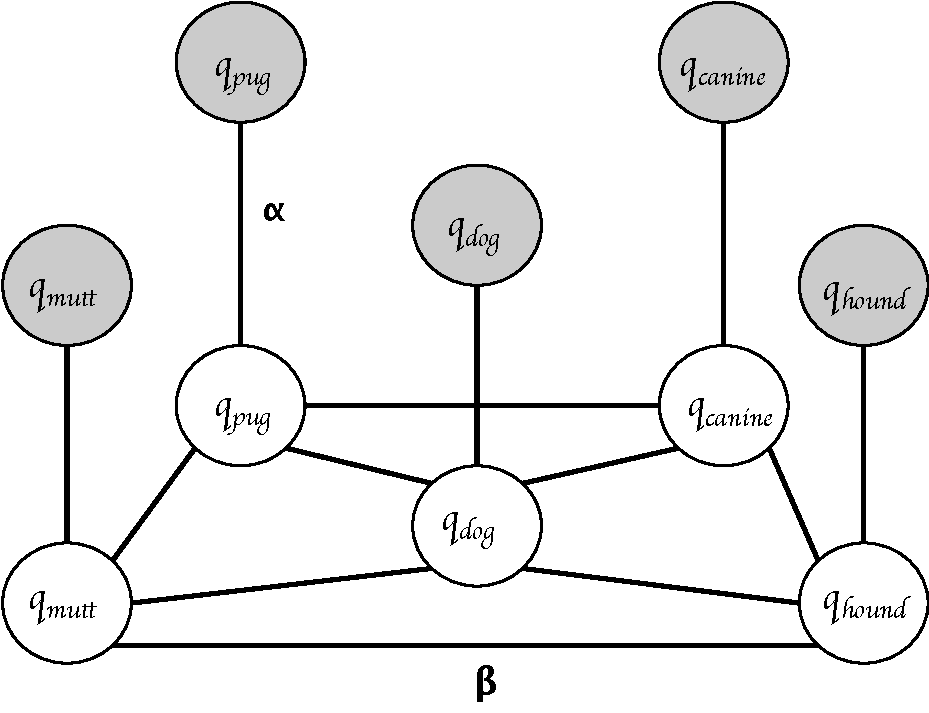
\includegraphics[width=\columnwidth]{diagram.png}
  \caption{Word graph with edges between related words showing the observed and the inferred word vector representations.}
  \label{fig:word-graph}
\end{figure}

Let $W = \{w_1,...,w_n\}$ be the set of word types and $\Sigma$ be an ontology that encodes a set of semantic relations between words in $W$. 
Specifically, we define $\Omega = (V_\Omega,E_\Omega)$ to be an undirected graph with vertices $V_\Omega = \{v_i | \  \forall \  w_i \in W\}$ and 
edges $E_\Omega = \{e_{ij}\}$ for every pair of words $(w_i,w_j)$ that are semantically linked \jdd{within $\Sigma$ } \cancel{according to different semantic relations}. These relations differ for different semantic lexicons as described later in~\S\ref{sec:lexicons}.
Since \jdd{the} majority of the existing word representation models ignore word-senses,
we consider \cancel{ $\forall i, w_i$} \jdd{$ w_i,\forall i$} to represent undisambiguated word-types; our model, however,
can be augmented to induce representations for sense-specific vectors as well (\S\ref{sec:word-sense}).

Then, given a set of word vectors $\hat{Q} = \{\hat{q}_i | \  \forall \  w_i \in W\}$ that have 
either been learned from any of the currently available
methods (described later in \S\ref{sec:vectors}) or are currently being learned, 
our objective is to learn a set of vectors $Q = \{q_i | \  \forall \  w_i \in W\}$ that are 
consistent with both $\hat{Q}$ and neighboring nodes in $\Omega$ by a notion of 
distance metric between vectors. 
Figure~\ref{fig:word-graph} shows a small word graph with such edge 
connections. The sets of nodes containing vectors $Q$ and vectors $\hat{Q}$ 
can be seen as the unobserved and observed nodes in a markov random field 
\cite{kindermann80mrf}. We initialize the vectors in $Q$ to be equal to the vectors in $\hat{Q}$
and then perform inference to obtain the unobserved (and retrofitted) word representations $Q$.

We define the distances between any two nodes as the euclidean distance\footnote{Theoretically, using negative cosine similarity as distance yields the same update equation for vectors of unit length}
 between their word vectors, thus forcing 
neighboring nodes to have similar vector representations. Since we want the inferred word vector \jdd{$q_i$} to be
associated both with its observed value $\hat{q}_i$ and its neighbors 
$q_j, \forall ij \in E_{\Omega}$, the objective becomes:
\begin{equation}
  \label{equ:eucl}
  \displaystyle \Psi(Q) = \sum_{i=1}^n \left[ \alpha_i \lVert q_i - \hat{q_i} \rVert^2 + \sum_{ij \in E_{\Omega}} \beta_{ij} \lVert q_i - q_j \rVert^2 \right]
\end{equation}
\jdd{I would rather the inner sum be like this: $\sum\limits_{j\in E_{\Omega_i}}$ so we're not looping over i twice. maybe there's a better solution with something like $\sum\limits_{j\in\{i,j\} s.t. e_{i,j}\in E_\Omega}$, which is more accurate but too long.}
where, $\beta_{ij}$ is the weight of the edges (details in \S\ref{sec:exp-post-proc}) 
connecting $i,j$ and $\alpha_i$ is a parameter to control the degree of deviation of the word 
vector from its observed value. We now look at two different ways of 
using this objective for retrofitting the vectors to semantic lexicons:
as a post-processing step after training the word vectors and during training the word vectors.

\subsection{Retrofitting by Post-processing}
\label{sec:post-proc}

In this \cancel{case}\jdd{approach}, we first train the word vectors independent of the information in the semantic lexicons
and \cancel{later} \jdd{then} retrofit them as a post-processing step. Equation~\ref{equ:eucl} is a convex 
optimization problem whose solution \cancel{is} \jdd{involves} solving a system of linear equations, \cancel{involving} \jdd{including} inversion of a 
large matrix which is $O(n^3)$; \cancel{thus} instead we use an iterative update \jdd{scheme} \cancel{schema} for 
optimization~\cite{Bengio+al-ssl-2006,Subramanya:2010:EGS:1870658.1870675,das-petrov:2011:ACL-HLT2011,das-smith:2011:ACL-HLT2011}.
We take the gradient of equation~\ref{equ:eucl} with respect to the parameters to be optimized, namely: \cancel{$\forall i, q_i$}\jdd{$q_i,\forall i$} and equate it to zero to get the following update\cancel{ for $q_i$}:
\begin{equation}
  \label{equ:update-vector}
q_i = \frac{\sum_{j, ij \in E} \beta_{ij} q_j + \alpha \hat{q_i}}{\sum_{j, ij \in E} \beta_{ij} + \alpha}
\end{equation}

In practice running this procedure for $10$ iterations leads to convergence. This is a simple 
post-processing model that can work with any kind of word vector representations.

\subsection{Bayesian Retrofitting}
\label{sec:during-training}

Training neural language models include performing maximum likelihood estimation (MLE) on the 
word vector parameters~\cite{Collobert:2008:UAN:1390156.1390177,MnihTeh2012,mikolov2013efficient}. 
These models maximize $p(w|h;Q)$, the probability of observing a word $w$ given a sequence of contextual words
$h$ and the word vectors $Q$. In addition to this, we formulate the information from the semantic lexicons
as a prior on the parameters $Q$ and instead perform a maximum a posteriori estimation (MAP). The prior
on $Q$ can be defined as:
\begin{equation}
  \label{equ:prior}
  p(Q) \propto \text{exp}\left(-\gamma\sum_{i=1}^{n}\sum_{ij \in E_{\Omega}}\beta_{ij} \lVert q_{i}-q_{j} \rVert^{2}\right)
\end{equation}
where $\gamma$ is a hyper-parameter that controls the strength of the prior. This prior on the word
vector parameters forces words connected in the lexicon to have close vector representations similar to
equation~\ref{equ:eucl}.

\subsection{Optimization}
\label{sec:optimization} 

The optimization of the objective during post-processing (\S\ref{sec:post-proc}) is a series of iterative
updates of the parameters $Q$. For the bayesian framework (\S\ref{sec:during-training}) we use two different
techniques for performing MAP. 

In the first technique, we take the derivative of the log prior (equ.~\ref{equ:prior}) with respect to the
parameters $Q$ and add it to the gradient of the posterior, thus optimizing them jointly
using adaptive gradient descent~\cite{Duchi:EECS-2010-24}.
However, since computing gradient of equ.~\ref{equ:prior}
is linear in the vocabulary size $n$, we use lazy updates~\cite{Carpenter08lazysparse} every
$k$ words during training i.e, if the gradient update for one training instance is $g$, the
lazy gradient would be $kg$ and would be computed after every $k$ training instances.
We call this the \textbf{XYZ} method of retrofitting during training.
The second technique is the stochastic gradient descent method of optimization 
while training. While optimizing the posterior $p(w|h;Q)$ we re-estimate the 
word vectors using equ.~\ref{equ:update-vector} after we visit every $k$ words during 
training. We call this the \textbf{ABC} method of retrofitting during training.

\section{Word Vector Representations}
\label{sec:vectors}

We test our retrofitting model on a number of different models of word vector
representations described below. We train some models on our data 
(\S\ref{sec:lsa},\S\ref{sec:sg},\S\ref{sec:lbl})
and use pre-trained vectors from other models (\S\ref{sec:gc},\S\ref{sec:multi}).

\subsection{Latent Semantic Analysis (LSA)}
\label{sec:lsa}

\jdd{To learn these word vectors, }we perform latent semantic analysis~\cite{deerwester-90} on a word-word co-occurrence matrix.
We construct a word co-occurrence frequency matrix for a given training corpus where
each row $\boldsymbol{w}$, represents one word in the corpus and every column $\boldsymbol{c}$, is the context 
feature in which the word is observed. In our case, every column is a word which occurs
in a given window length around the target word. For scalability reasons, we
only select words with frequency greater than $10$ as features. We also remove
the top $100$ most frequent words (mostly stop words) from the column features.

We then replace every entry in the sparse frequency matrix by 
its pointwise mutual information (PMI) \cite{Church:1990:WAN:89086.89095,Turney:2001:MWS:645328.650004}
resulting in $\boldsymbol{X}$.
We factorize the matrix $\boldsymbol{X} = \boldsymbol{U} \boldsymbol{\Sigma} \boldsymbol{V}^{\top}$ using singular value decomposition (SVD)~\cite{Golub:1996:MC:248979}. Finally, we obtain a reduced dimensional
representation of words from size $O(n)$ to $k$ by selecting the first $k$ columns of $\boldsymbol{U}$.

\subsection{Skip-gram Vectors (SG)}
\label{sec:sg}

\jdd{The} \texttt{Word2Vec} word vector tool~\cite{mikolov2013efficient} is currently the fastest and 
the most \jdd{widely-}used tool for obtaining word 
vector representations from an unlabeled 
corpus.\footnote{\url{https://code.google.com/p/word2vec/}}
Every word in the skip-gram model is represented by its Huffman code~\cite{citeulike:1320251}. In 
this model, each \cancel{current} word is used as an input to a log-linear classifier
with continuous projection layer and words within a certain range before and after the word
are predicted. 

\subsection{Global Context Vectors (GC)}
\label{sec:gc}

These word vectors~\cite{huang2012improving} have been created using a neural network model which not only takes the local context of the word into account but also uses global features extracted at the document level to further enrich the vector quality.\footnote{\url{http://nlp.stanford.edu/~socherr/ACL2012_wordVectorsTextFile.zip}}

\subsection{Multilingual Vectors (Multi)}
\label{sec:multi}

These word vectors~\cite{faruqui-dyer:2014:EACL2014} have been created using spectral learning where the authors first create monolingual word vectors by performing SVD on a monolingual word co-occurrence matrix and then use canonical correlation analysis (CCA) on pairs of vectors from different languages to obtain improved vector representations.\footnote{\url{http://www.wordvectors.org/web-eacl14-vectors/de-projected-en-512.txt.gz}}

\subsection{Log-bilinear Vectors (LBL)}
\label{sec:lbl}

The log bilinear language model~\cite{MnihTeh2012} predicts a word given its
context. \cancel{ where every word } \jdd{maybe this commented out line wasn't supposed to be commented out?}
%$w$ is represented by a word vector $q_w$ and a bias $b_w$ which constitute the parameters $\theta$ of the model. 
If $h$ is set of context words, then the association between the target word 
and the context is defined
as $s(w, h;Q) = \sum_{w_i \in h}q_{w}^{\top}q_{w_{i}} + b_{w_{i}}$. Thus, the probability of observing $w$ given $h$ is:
\begin{equation}
  \label{equ:prob-lbl}
  p(w|h;Q) = \frac{\text{exp}(s(w, h;Q))}{\sum_{i=1}^{n}\text{exp}(s(w_{i}, h;Q))}
\end{equation}
Since, it is very costly to marginalize the socre over the whole vocabulary, 
we use \textit{noise constrastive estimation} (NCE) to estimate the parameters 
of the model~\cite{MnihTeh2012} using AdaGrad~\cite{Duchi:EECS-2010-24} with a 
learning rate of $0.05$.
%\footnote{We implemented this model ourselves as the code is not publicly available}

\section{Semantic Lexicons}
\label{sec:lexicons}

\jdd{In this section, we describe the three lexical ontologies used in our experiments. These ontologies were simple to fit into our approach, but this technique can be easily extended to any ontology which encodes relations between word types.} We use three different semantic lexicons to evaluate their utility in improving
the word vectors.
% and then merge them all together to act as a single large ontological resource.

\subsection{Paraphrase Database} 
\label{sec:ppdb}

The paraphrase database (PPDB) \cite{ganitkevitch2013ppdb} is a semantic lexicon containing more than 220 million paraphrase pairs of English, including 8 million lexical paraphrases, i.e. paraphrases of length 1. It has been constructed by pivoting words across multiple languages. The key concept behind obtaining lexical paraphrases through pivoting is that words of one language that are aligned to the same word in a different language should be synonymous. For example, if the words \textit{jailed} and \textit{imprisoned} map to the same word in another language, it may be reasonable to assume they have the same meaning. For our experiments, for each lexical paraphrase in PPDB, there exists an edge in our graph. The lexical paraphrase dataset comes in different sizes ranging from S to XXXL, in decreasing order of paraphrasing confidence and increasing order of size. We chose XL size for our experiments that produces a graph of $103,000$ nodes and $230,000$ edges\footnote{\url{http://www.cis.upenn.edu/~ccb/ppdb/}}.
Since, PPDB is an automatically created ontology, it has confidence score for a word being 
paraphrased into another word. We conduct two sets of 
experiments using the 
PPDB: (1) The $\alpha$s in equation \ref{equ:euc} are set to 1, (2) The $\alpha$s in \ref{equ:euc} are set to the weights from PPDB(cf. \S\ref{sec:expts}). 

\subsection{WordNet} 
\label{sec:wordnet}

WordNet~\cite{miller:1995} is a large, hand-annotated semantic lexicon of English words. 
It groups English words into sets of synonyms called synsets, provides short, general definitions, and records the various semantic relations between these synonym sets.
This database is structured in a graph particularly suitable for our task because it explicitly relates concepts with semantically aligned relations such as hypernyms and hyponyms. For example, the word \textit{dog} has a synonym \textit{canine}, a hypernym \textit{puppy} and a hyponym \textit{animal}. We perform two different experiments with WordNet where a given word is connected to \jdd{either}
its (1) synonyms, \jdd{or} (2) synonyms, hypernyms, and hyponyms. 
\jdd{Using this ontology,} we get a graph of $148,000$ nodes and $560,000$ edges. \jdd{Which setup gives us this number of edges? They must vary between WordNet and WordNet++, which are outlined here.}

\subsection{FrameNet}
\label{sec:framenet}

FrameNet~\cite{fillmore-ua-2003} is a rich linguistic resource containing  information about
lexical and predicate-argument semantics in English. Grounded in the theory of frame semantics, it suggests 
a semantic representation that blends word-sense disambiguation and semantic role labeling. The FrameNet lexicon
\cite{Baker:1998:BFP:980845.980860} is a taxonomy of manually identified general-purpose frames for English. 
Listed in the lexicon with each frame are several lemmas that can denote the frame or some aspect of it. 
We use this grouping of words in a particular frame as evidence that these words are semantically related and
connect all words in one frame to each other in our word graph. For example, the frame \texttt{CAUSE CHANGE POSITION ON A SCALE} contains words \textit{push, raise} and \textit{growth}. \jdd{Using this ontology,} we get a graph of $11,000$ nodes and $210,000$ edges. 

\section{Evaluation Benchmarks}
\label{sec:eval}

We evaluate the quality of our word vector representations on tasks that
test how well they capture both semantic and syntactic aspects of the representations
along with an extrinsic sentiment analysis task.

\subsection{Word Similarity}
\label{sec:word-sim}

We evaluate our word representations on a variety of different benchmarks that
have been widely used to measure word similarity. The first \cancel{one} is the \textbf{WS-353}
dataset~\cite{citeulike:379845}, containing 353 pairs of English words that have been 
assigned similarity ratings by humans. The second \cancel{benchmark} is the \textbf{RG-65} 
\cite{Rubenstein:1965:CCS:365628.365657} dataset, \cancel{that contain} \jdd{containing} 65 pairs of nouns. 
Since the commonly used word similarity datasets contain a small number of word pairs we
also use the \textbf{MEN} dataset~\cite{bruni:2012} that contains $3000$ word 
pairs which have been sampled from words
that occur at least $700$ times in a large web corpus. 

We calculate similarity between a given pair of words by the \textit{cosine}
similarity between their corresponding vector representation.
We then report Spearman's rank correlation coefficient 
\cite{citeulike:8703893} between the rankings produced by our model against the human rankings.

\begin{comment}
\subsection{Sentence Completion (SENT)}
The Microsoft Research sentence completion dataset contains $1040$ sentences
from each of which one word has been removed. The task is to correctly predict
the missing word from a given list of $5$ other words per sentence. We average
the word vectors of a given sentence $q_{sent} = \sum_{i=1, i\neq j}^{N} q_{w_i}/N$, where
$w_j$ is the missing word and 
compute the cosine similarity of $q_{sent}$
vector with each of the options. The word with the highest similarity is chosen
as the missing word placeholder.
\end{comment}

\subsection{Syntactic Relations (SYN-REL)}
\label{sec:syn-rel}

\newcite{mikolov-yih-zweig:2013:NAACL-HLT} present a new syntactic relation dataset composed of analogous word pairs. 
It contains pairs of tuples of word relations that follow a common syntatic relation. For example, in \textit{walking} and \textit{walked}, the second word is the past tense \jdd{form}
of the first word. There are nine such different kinds of relations: adjective-adverb,
opposites, comaparative, superlative, present-participle, 
nation-nationality, past tense, plural nouns and plural verbs.
Overall there are $10675$ such syntactic pairs of word tuples.

The task here is to find a word \textit{d} that best fits the following relationship: 
\textit{a~:~b~::~c~:~d} given \textit{a, b} and \textit{c}. 
We use the vector offset method described in 
\newcite{mikolov2013efficient} that computes the vector $q = q_a - q_b + q_c$ where, 
 and return the 
vector $q_w$ from the whole vocabulary which has the highest cosine similarity to $q$.
%\begin{equation}
%q_w = \underset{q_w}{\argmax}\frac{q_w \cdot q}{\left| q_w \right| \cdot \left| q \right|}
%\end{equation}
%It is worth noting that this is a non-trivial $n$-way classification task
%where $n$ is the size of the vocabulary.

\subsection{Synonym Selection (TOEFL)}
\label{ref:toefl}

The synonym selection task is to select the semantically closest word to a target from a list of candidates. The dataset we use on this task is the TOEFL dataset \cite{landauer:1997} which consists of a list of target words that appear with 4 candidate lexical substitutes each. The dataset contains 80 such questions. An example is ``\textit{rug $\rightarrow$ sofa, ottoman, carpet, hallway}'', with ``\textit{carpet}'' being the most synonym-like candidate to the target.

\subsection{Sentiment Analysis (SA)}
\label{sec:senti}

\newcite{Socher-etal:2013} have created a treebank which contains sentences
annotated with fine-grained sentiment labels on both the phrase and sentence level
and show that compositional vector space models can be used to predict sentiment
at these levels with high accuracy.
These sentences are movie review excerpts originally collected by \newcite{Pang:2005:SSE:1219840.1219855}.
The coarse-grained treebank, containing only positive and negative 
classes has been split into training, development and test datasets containing $6920$, $872$ and 
$1821$ sentences respectively. We train a logistic regression classifier with $L2$ regularization
on the average of the word 
vectors of a given sentence to predict the coarse-grained sentiment tag at the sentence level.

\section{Experiments \& Results}
\label{sec:expts}

We train word vectors of length $80$ for the LSA (\S\ref{sec:lsa}), log bilinear (\S\ref{sec:lbl}) 
and the skip-gram (\S\ref{sec:sg}) vectors. The corpus used was the monolingual English news corpus from 
WMT-2011.\footnote{\url{http://www.statmt.org/wmt11/}} After normalization the corpus 
contained $360$ million word tokens and $180,000$ word types. For the global context 
(\S\ref{sec:gc}) and the Multilingual (\S\ref{sec:multi}) vectors
we use the word vectors available on the website.
We ran experiments showing that our model can be used to retrofit the word vectors both
as a post-processing step or during training.

\subsection{Retrofitting by Post-processing}
\label{sec:exp-post-proc}

We use equ.~\ref{equ:update-vector} to optimize word vectors using different 
semantic lexicons under different settings as described below. \jdd{The structure of the ontology chosen informs the structure of the graph used in our optimization procedure.}

\paragraph{PPDB.} There exists an edge between a word and all its paraphrases \jdd{in PPDB}. For every word $w_i$, we set $\alpha_i = 1$ and the edge weight for every neighbor $\forall j, \beta_{ij} = 1/N$, where $N$ is the number of neighbors of the word. This \jdd{ensures} \cancel{makes sure} that the optimized word vector is still not very far from its originally observed estimate.

\paragraph{wtPPDB.} PPDB has weights associated with every paraphrase word pair $p(w_i | w_j)$ and $p(w_j |w_i)$ which are the conditional probabilities of 
observing the paraphrase given the word and vice versa obtained empirically during the construction of the PPDB. We define $\forall j, \beta_{ij} = p(w_i | w_j)/2 + p(w_j |w_i)/2$ and keep $\alpha_i = 1$ as in the previous experiment. 

\paragraph{WN.} There exists an edge between a word and all of its synonyms \jdd{in WordNet}. 
For every word $w_i$, we set $\alpha_i = 1$ and the edge weight for every neighbor 
$\forall j, \beta_{ij} = 1/N$, where $N$ is the number of neighbors of the word. 

\paragraph{WN++.} There exists an edge between a word and all of its synonyms, 
hypernyms and hyponyms \jdd{in WordNet}. For every word $w_i$, we set $\alpha_i = 1$ and the edge weight
for every neighbor $\forall j, \beta_{ij} = 1/N$, where $N$ is the number of neighbors of the word. 

\paragraph{FN.} There exists an edge between all the words that evoke the same 
semantic frame \jdd{in FrameNet}. For every word $w_i$, we set $\alpha_i = 1$ and the edge weight
for every neighbor $\forall j, \beta_{ij} = 1/N$, where $N$ is the number of neighbors of the word. 

\paragraph{Results.} Figure~\ref{fig:post-proc} shows the absolute improvements
in both the spearman's correlation ratio and the accuracy obtained on different
tasks over the baseline. Every row of plots shows one semantic lexicon being used
for retrofitting \jdd{, while every column shows one evaluation task}. The different vector models are shown in different colors. 

We see that all the lexicons are helpful in improving
the Spearman's correlation ratio in the word similarity tasks. However, FrameNet is
either not improving the results or \cancel{even} making them worse in many cases (\cancel{for example} \jdd{e.g.} the skip-gram and multilingual vectors). In the syntactic relation task (\S\ref{sec:syn-rel}), 
we get huge improvements \cancel{of} \jdd{on} the order of $10$ absolute points
in accuracy for all ontologies except for FrameNet. For the extrinsic sentiment analysis task (\S\ref{sec:senti}) we get improvements using all the ontologies and achieve the highest improvement of absolute $1.4$ points in accuracy for the multilingual vectors over the baseline (\S\ref{sec:multi}). \jdd{Though not as large as on the other tasks, this gain} 
is statistically significant ($p<0.01$) according to a McNemar's test~\cite{Dietterich98approximatestatistical}.

Interestingly, \textbf{wtPPDB} is \jdd{not better} \cancel{almost as good as or even worse} than 
the uniformly weighted \textbf{PPDB} 
setting which signifies that PPDB already has a highly confident
set of paraphrases which are of equal quality. 
Also, the reason that FrameNet does not perform as well as the other 
ontologies may be because words of significantly different meaning can evoke the 
same frame. For example, \textit{push} and \textit{growth} are two words of 
different meanings but they evoke the same frame as described in \S\ref{sec:framenet}.
Overall, we observe that \textbf{PPDB} helps in improving the quality of the word vectors
irrespective of the type of task and the word vector model.

\paragraph{Lexicon Ensemble.} We now examine if we can combine multiple ontologies
together in a way which can lead to performance gain more than either of these ontologies alone.
We perform two experiments, in the first experiment we take a union of the sets of edges 
of the two lexicons and in the second experiment we take the intersection of the
sets of edges.
We then perform retrofitting of vectors using the new lexicon and carry out the evaluation.
As can be expected, taking union of ontologies performed better than taking 
intersection and hence we only show the union results in the bottom 
row of figure~\ref{fig:post-proc}. We only explore the union of WordNet and 
PPDB and exclude FrameNet as it did not give positive results on its own. \jdd{We should move this to where we're describing how we've made all of the graphs, immediately after the ``FN'' paragraph.  It should be titled ``Union'' and should be described in the same way as the other graph generation procedures. We can still say we took the union of the best two ontologies, and that the intersection didn't help, but this paragraph should be with those others.}

\begin{figure*}[!tb]
  \centering
  \includegraphics[width=2\columnwidth]{plots_weighted_ppdb_wordnet.pdf}
  \caption{Absolute improvement in \cancel{the} Spearman's correlation ratio (3 left columns) and accuracy (3 right 
  columns) using different semantic lexicons on different tasks. \jdd{Comparing vertically shows which ontologies perform better. }}
  \label{fig:post-proc}
\end{figure*}

\subsection{Retrofitting while Training}
\label{sec:improve-tr}

\begin{table*}[!tbh]
  \centering
  \small
  \begin{tabular}{l|c||c|c|c||c|c||c}
Method & $k$/$\gamma$ & WS-353 & RG-65 & MEN & SYN-REL & TOEFL & SA \\
\hline
Baseline & $k=\infty$, $\gamma=0$ & 53.6 & 42.7 & 58.0 & 31.5 & 66.7 & 72.5 \\
\hline
\multirow{3}{*}{XYZ} & $\gamma=1$ & 54.2 & 46.9 & 57.6 & 32.1 & 66.6 & \textbf{73.7}\\
 & $\gamma=0.1$ & 54.0 & 50.8 & 58.7 & 32.2 & 65.3 & 73.3\\
 & $\gamma=0.01$ & \textbf{55.3} & \textbf{52.2} & \textbf{58.7} & \textbf{33.4} & \textbf{69.3} & 72.9\\
\hline\hline
\multirow{3}{*}{ABC} & $k=100m$ & 57.2 & 61.1 & \textbf{61.8} & \textbf{36.3} & 78.7 & 73.8\\
 & $k=50m$ & \textbf{58.0} & \textbf{62.2} & 61.4 & 32.1 & 85.3 & \textbf{74.4} \\
 & $k=25m$ & 56.3 & 60.8 & 58.5 & 27.8 & \textbf{88.0} & 73.3\\
\end{tabular}
   \caption{%Enrichment while training of LBL word embeddings using PPDB.
   Spearman's correlation (3 left columns) and accuracy (3 right columns) on different tasks. Bold indicates 
   best result across all vector types.}
  \label{tab:lbl-tr}
\end{table*}

We now discuss the experiments of retrofitting while training the word vectors. Note that
for this we need to alter the training algorithm and hence we conducted experiments only
with the log bilinear model (\S\ref{sec:lbl}) for which we implemented the model training ourselves.
We conduct experiments for both \textbf{XYZ} and \textbf{ABC} algorithms of
MAP estimation. For the \textbf{XYZ} method
we update the prior every $k=100,000$ words\footnote{Experiments with $k \in [10000, 50000]$ 
yielded almost similar results.} and test for different values of $\gamma \in [1, 0.1, 0.01]$.
For the \textbf{ABC} method, we update the word vectors using equ.~\ref{equ:update-vector}
every $k*10^6, k \in [25, 50, 100]$ words. 

Table~\ref{tab:lbl-tr} shows the results of improvement while training word vectors of length $80$. 
We show experimental results 
with only PPDB (\S\ref{sec:ppdb}) as the ontology. For \textbf{XYZ}
$\gamma = 0.01$ performs the best although other values of $\gamma$ also yield very close 
results. For \textbf{ABC} \cancel{$k=50$}\jdd{$k=5*10^6$} perform the best although all other values of $k$
also perform better than the baseline. Overall we see that the both the methods lead to 
improvement in performance across all tasks however \textbf{ABC} is relatively better in
performance. \jdd{We have to have at least a sentence or two comparing these results to the improvement in the table above it. We can say something like ``We see similar gains, which aren't as large as in post processing.''}

\subsection{Multilingual Evaluation}
\label{sec:multilingual}

\begin{figure}[!tb]
  \centering
  \includegraphics[width=1\columnwidth]{multi-plot.png}
  \caption{Improvement in spearman's correlation for word similarity evaluation using the
  retrofitted vectors from different word vector models on French (WS-353), German (RG-65)
  and Spanish (MC-30).}
  \label{fig:multi-lang}
\end{figure}

We tested our method on three different languages other than English: German,
French and Spanish. We used the Universal WordNet \cite{deMeloWeikum2009}, which 
is an automatically constructed multilingual lexical knowledge base based on 
WordNet.\footnote{\url{http://www.mpi-inf.mpg.de/yago-naga/uwn/}} 
It contains words connected via different lexical relations to other words both
in and across languages. For a word in a language we only consider links going to
the other words in the same language to construct the word graph. We first train
word vectors for these three languages and then improve them using the ontological
information.

For German, French and Spanish we constructed word graphs containing around $87000$, $49000$
and $31000$ word nodes being connected to other nodes via $200000$, $100000$ and $52000$ 
edges respectively. 
Since not many word similarity evaluation benchmarks are available for other languages 
we tested our baseline and improved vectors on one benchmark per language.
We used RG-65 \cite{Gurevych:2005:USC:2145899.2145986}, WS-353 \cite{Joubarne:2011:CSS:2018192.2018218} 
and MC-30 \cite{Hassan:2009:CSR:1699648.1699665} for German, French and Spanish respectively. 
We trained three different types of vectors: LSA (\S\ref{sec:lsa}), Skip-Gram (\S\ref{sec:sg})
and LBL (\S\ref{sec:lbl}) for all the three languages of length 80 while keeping all other parameters
same as previously described. We again used the WMT-2011 monolingual news corpus for all the 
languages and evaluate word similarity on these tasks before and after enrichment. 
Figure~\ref{fig:multi-lang} shows the results that strongly 
indicate that our method generalizes across languages. We get high improvements in the 
Spearman's correlation coefficient on the word similarity tasks for the three languages for three
different kinds of vectors.

\section{Sense Specific Vectors?}
\label{sec:word-sense}

\begin{figure}[tb]
  \centering
  \includegraphics[width=\columnwidth]{multi-sense.png}
  \caption{Word graph for inducing sense-specific vectors from a sense-agnostic word vector model.}
  \label{fig:sense-graph}
\end{figure}

\jdd{I would remove the question mark from the title. I think this is a good step towards learning sense-specific vectors, and lays the groundwork for future research.}
Most word vector models assign one vector to each word type
ignoring the possibility that the same word type may have more than one meaning. 
Should an obviously polysemous word like \textit{bank} really be represented using
the same structure (i.e, a single vector) as a more monosemous word \textit{anger}?
Two previous efforts have attempted to learn sense-specific vectors by 
clustering contexts to discriminate
word senses into multiple prototype vectors~\cite{reisinger:naacl10,huang2012improving}. 
However, the resulting vectors
lack interpretability and cannot be matched to senses present in a lexicon \jdd{such as Wordnet}\cancel{
for ex., WordNet}.

We augment our retrofitting framework (\S\ref{sec:framework}) using WordNet, \jdd{which}
\cancel{that} provides information about the number of senses for a particular word
and its \jdd{synonyms} \cancel{synset (synonym set)}. We introduce an unobserved node for every sense of a 
word and connect all of them to one observed node in the graph, which represents the word
vector obtained for that word from a word vector model. We then connect
each of these nodes to \cancel{other words in its synset}\jdd{it's synonyms} in the regular manner. 
For example, in figure~\ref{fig:sense-graph}, for the word \textit{bank}, 
if we have two senses in the WordNet,
we create two unobserved nodes each connected to the observed node representing
the word vector $\hat{q}_{bank}$ and also connected to other words in their respective 
synset.
Now performing belief propagation on this graph as a simple post-processing step
(\S\ref{sec:post-proc}) gives us the sense specific vector corresponding to each
sense in the WordNet. 
%This makes the vectors being more interpretable in terms of exactly which sense it represents.
Intuitively the sense-laebeled vectors ``pull apart'' the components of the 
sense-agnostic vectors.

\begin{table*}[ht]
\begin{center}
\begin{small}
\begin{tabular}{|c|ccc|}
\hline 
Word or Word Sense & \multicolumn{3}{c|}{Top 3 Most Similar Words or Word Senses}\tabularnewline
\hline 
hanging & hung & dangled & hangs\tabularnewline
hanging\%1:04:01:: (act of suspending something) & shoring\%1:04:00:: & support\%1:04:01:: & suspension\%1:04:00::\tabularnewline
hanging\%1:06:00:: (decoration hung on a wall) & tapestry\%1:06:00:: & braid\%2:35:01:: & smock\%2:36:00::\tabularnewline
\hline 
crossbar & left-foot & left-footed & header\tabularnewline
crossbar\%1:06:01:: (game equipment horizontal bar) & header\%1:06:00:: & equalizer\%1:06:01:: & goalie\%1:18:00::\tabularnewline
crossbar\%1:06:02:: (horizontal bar across something) & shackle\%1:06:01:: & heaver\%1:06:00:: & bar\%1:06:00::\tabularnewline
\hline 
climber & climbers & skier & Loretan\tabularnewline
climber\%1:18:00:: (someone who climbs as a sport) & lifter\%1:18:00:: & swinger\%1:18:01:: & sharpshooter\%1:18:01::\tabularnewline
climber\%1:20:00:: (a vine or climbing plant) & woodbine\%1:20:02:: & brier\%1:20:02:: & kiwi\%1:20:00::\tabularnewline
\hline 
\end{tabular}
\end{small}
\caption{The top 3 most similar words or word senses for some polysemous words. WordNet definitions for word senses are given in brackets where appropriate. 
%Single sense VSMs largely capture the most frequent sense. Our technique effectively separates out the different senses of words and produces meaningful sense-specific vectors.
}\label{tbl:mostsim}
\end{center}
\end{table*}

In table \ref{tbl:mostsim} we present some analysis that qualitatively \cancel{attempts to evaluate} \jdd{evaluates} the nature of 
sense-specific word vectors. The table shows the three most similar words of an ambiguous word in standard SG model (\S\ref{sec:sg}) in comparison with the three most similar words of different word senses of the same word in the disambiguated SG model. 
The standard vector models %almost always capture only the 
are either dominated by the most frequent sense or they mix multiple senses of a word. 
On the other hand, the disambiguated vectors appear to capture sense specificity of less frequent senses successfully. The examples in table \ref{tbl:mostsim}, while chosen for their prominence in evidencing the phenomenon, are fairly representative of the whole vector space in general. We propose to carry out
extensive quantitative evaluation of the sense-specific vectors as future work.
%We noticed that lemma senses that had many neighbors (i.e. synonyms, hypernyms and hyponyms), tended to have more clearly sense specific vectors --- as measured by their cloud of most similar senses. This is expected, since it is these neighborhoods that disambiguate and help to distinguish the vectors of less frequent word senses from their single sense empirical embeddings.
%We believe that the \emph{ordering} of the semantic space as a result of the ontological graph smoothing procedure is the reason for the consistently better results we showed in section \ref{sec:evaluation}.

\section{Related Work}

In terms of methodology, the approach we propose is conceptually similar to previous work that leverages graph 
structures to propagate information among semantic concepts~\cite{Zhu:2005:SLG:1104523,10.1109/TPAMI.2007.70765}. 
%Most notably, \newcite{das-smith:2011:ACL-HLT2011} 
%construct a factor graph of a semantic lexicon that is used to generalize and apply semantic frames to %previously unseen types. 
Graph based belief propagation has also been used to induce POS tags
\cite{Subramanya:2010:EGS:1870658.1870675,das-petrov:2011:ACL-HLT2011}
and semantic frame induction \cite{das-smith:2011:ACL-HLT2011} both of
which use belief propagation in a manner similar to ours to obtain
labels for unknown words.
%Our approach is closest to \newcite{das-petrov:2011:ACL-HLT2011} who induce POS tag distribution
%for words in a resource poor language through a resource rich language but differs in that we induce
%monolingual word vector representations instead of POS tag distributions.

The use of lexical semantic information in training word vectors has been limited. 
Recently, \newcite{Yu:2014} used semantic knowledge to improve the 
Word2Vec~\cite{mikolov2013efficient}
embeddings in a joint training model similar to our retrofitting while 
training approach (\S\ref{sec:during-training}). 
\newcite{alfonseca:2002} attempt to extend an ontology such as WordNet with unsupervised and 
domain-specific information that is yielded by distributional vectors. 
%In contrast, \newcite{gabrilovich:2009} directly construct an ontology of concepts based on the Wikipedia knowledge-graph using a technique called Explicit Semantic Analysis which heavily relies on distributional statistics. 
\newcite{agirre:2001} enrich the 
WordNet ontology with topic rather than raw distributional signatures and \newcite{agirre:2013} use the WordNet 
graph to perform random-walks that guide a word-sense disambiguation process.

Word vectors have also shown to improve using cross lingual information both during
training \cite{zou-EtAl:2013:EMNLP,hermann2014multilingual} and as a post-processing operation \cite{faruqui-dyer:2014:EACL2014}.  
%and dependency based context \cite{Pado:2007:DCS:1268656.1268658}. 
There have also been disparate attempts at enhancing distributional semantic representations with various sources of non-linguistic information such as images \cite{bruni:2011} and experiential data \cite{andrews:2009}.

Our approach of learning better word vector representations can be seen as an instance of graph based
semi-supervised learning~\cite{Zhu:2005:SLG:1104523,Talukdar:2010:EGS:1858681.1858830} 
where the supervision is derived from the explicit word relations in Semantic Lexicons. Graph based
learning has also been employed in machine translation \cite{Alexandrescu:2009:GLS:1620754.1620772,saluja:2014:ACL2014},
unsupervised semantic role induction \cite{Lang:2011:USR:2145432.2145571}, 
semantic document modeling~\cite{schuhmacher:2014}, 
language generation~\cite{Krahmer:2003:GGR:778822.778825} and
sentiment analysis~\cite{Goldberg:2006:SSA:1654758.1654769}.

\section{Conclusion}

We have proposed a simple and effective method to improve
word vectors (obtained from different models of word representations)
using either automatically or human constructed semantic lexicons
that have explicit information about word relations. We have shown that
retrofitting the word vectors to semantic lexicons is useful and 
can be performed both during training
the word vectors or as a post-processing operation. We validated the
applicability of our method across a number of languages and showed that 
performance improvement can be obtained on different types of evaluation tasks.

\bibliography{references}
\bibliographystyle{acl}
\end{document}
